\documentclass[11pt]{article}

\usepackage{fullpage}
\parindent=0in


%------------------------------------------------------------------
% PROBLEM, PART, AND POINT COUNTING...

% Create the problem number counter.  Initialize to zero.
\newcounter{problemnum}

% Specify that problems should be labeled with arabic numerals.
\renewcommand{\theproblemnum}{\arabic{problemnum}}


% Create the part-within-a-problem counter, "within" the problem counter.
% This counter resets to zero automatically every time the PROBLEMNUM counter
% is incremented.
\newcounter{partnum}[problemnum]

% Specify that parts should be labeled with lowercase letters.
\renewcommand{\thepartnum}{\alph{partnum}}

% Make a counter to keep track of total points assigned to problems...
\newcounter{totalpoints}

% Make counters to keep track of points for parts...
\newcounter{curprobpts}		% Points assigned for the problem as a whole.
\newcounter{totalparts}		% Total points assigned to the various parts.

% Make a counter to keep track of the number of points on each page...
\newcounter{pagepoints}
% This counter is reset each time a page is printed.

% This "program" keeps track of how many points appear on each page, so that
% the total can be printed on the page itself.  Points are added to the total
% for a page when the PART (not the problem) they are assigned to is specified.
% When a problem without parts appears, the PAGEPOINTS are incremented directly
% from the problem as a whole (CURPROBPTS).


%---------------------------------------------------------------------------


% The \problem environment first checks the information about the previous
% problem.  If no parts appeared (or if they were all assigned zero points,
% then it increments TOTALPOINTS directly from CURPROBPTS, the points assigned
% to the last problem as a whole.  If the last problem did contain parts, it
% checks to make sure that their point values total up to the correct sum.
% It then puts the problem number on the page, along with the points assigned
% to it.

\newenvironment{problem}[1]{
% STATEMENTS TO BE EXECUTED WHEN A NEW PROBLEM IS BEGUN:
%
% Increment the problem number counter, and set the current \ref value to that
% number.
\refstepcounter{problemnum}
%
% Add some vspace to separate from the last problem.
\vspace{0.15in} \par
%
\setcounter{curprobpts}{#1} \setcounter{totalparts}{0}	% Reset counters.
%
% Now put in the "announcement" on the page.
{\Large \bf \theproblemnum. \normalsize ({\it \arabic{curprobpts} point\null\ifnum \value{curprobpts} = 1\else s\fi}\/)}
}{
% STATEMENTS TO BE EXECUTED WHEN AN OLD PROBLEM IS ENDED:
%
% If no parts to problem, then increment TOTALPOINTS and PAGEPOINTS for the
% entire problem at once.
\ifnum \value{totalparts} = 0
	\addtocounter{totalpoints}{\value{curprobpts}}	% Add pts to total.
	\addtocounter{pagepoints}{\value{curprobpts}}	% Add pts to page total.
%
% If there were parts for the problem, then check to make sure they total up
% to the same number of points that the problem is worth. Issue a warning
% if not.
\else \ifnum \value{totalparts} = \value{curprobpts}
	\else \typeout{}
	\typeout{!!!!!!!   POINT ACCOUNTING ERROR   !!!!!!!!}
	\typeout{PROBLEM [\theproblemnum] WAS ALLOCATED \arabic{curprobpts} POINTS,}
	\typeout{BUT CONTAINS PARTS TOTALLING \arabic{totalparts} POINTS!}
	\typeout{}
	\fi
\fi
}


%---------------------------------------------------------------------------


% The \newpart command increments the part counter and displays an appropriate
% lowercase letter to mark the part.  It adds points to the point counter
% immediately.  If 0 points are specified, no point announcement is made.
% Otherwise, the announcement is in scriptsize italics.

\newcommand{\newpart}[1]
{
\refstepcounter{partnum}	% Set the current \ref value to the part number.
%\hspace{0.25in}		% Indent the part by a quarter inch.
%
% If points are to be printed for this problem (signaled by point value > 0),
% then put them in in scriptsize italics.
\ifnum #1 > 0
	\makebox[0.25in][l]{{\bf \thepartnum.} {\bf ({\it #1 pt\ifnum #1 = 1\else s\fi\/}) \,\,}}
\else
	\makebox[0.25in][l]{({\bf \thepartnum})}
\fi
%
\hspace{0.1in}		% Lead the material away from the part "number".
%
\addtocounter{totalparts}{#1}	% Add points to totalparts for this problem.
\addtocounter{pagepoints}{#1}	% Add points to total for this page.
\addtocounter{totalpoints}{#1}	% Add points to total for entire test.
}


%---------------------------------------------------------------------------



% Just in case you want to skip some numbers in your test...

\newcommand{\skipproblem}[1]{\addtocounter{problemnum}{#1}}



%---------------------------------------------------------------------------


% The \showpoints command simply gives a count of the total points read in up to
% the location at which the command is placed.  Typically, one places one
% \showpoints command at the end of the latex file, just prior to the
% \end{document} command.  It can appear elsewhere, however.

\newcommand{\showpoints}
{
\typeout{}
\typeout{====> A TOTAL OF \arabic{totalpoints} POINTS WERE READ.}
\typeout{}
}


%---------------------------------------------------------------------------



\usepackage{graphicx}
\usepackage[english]{babel}
\usepackage[latin1]{inputenc}
\usepackage{times}
\usepackage[T1]{fontenc}
\usepackage{inconsolata}
\usepackage{amsmath}
\usepackage{amssymb}
\usepackage{hyperref}
\usepackage{color}

\newcommand{\argmax}{\mathop{\arg\max}}
\newcommand{\deriv}[1]{\frac{\partial}{\partial {#1}} }
\newcommand{\dsep}{\mbox{dsep}}
\newcommand{\Pa}{\mathop{Pa}}
\newcommand{\ND}{\mbox{ND}}
\newcommand{\De}{\mbox{De}}
\newcommand{\Ch}{\mbox{Ch}}
\newcommand{\graphG}{{\mathcal{G}}}
\newcommand{\graphH}{{\mathcal{H}}}
\newcommand{\setA}{\mathcal{A}}
\newcommand{\setB}{\mathcal{B}}
\newcommand{\setS}{\mathcal{S}}
\newcommand{\setV}{\mathcal{V}}
\DeclareMathOperator*{\union}{\bigcup}
\DeclareMathOperator*{\intersection}{\bigcap}
\DeclareMathOperator*{\Val}{Val}
\newcommand{\mbf}[1]{{\mathbf{#1}}}
\newcommand{\eq}{\!=\!}

\DeclareMathOperator*{\argmin}{arg\,min}
\DeclareMathOperator*{\sign}{sign}


\begin{document}

{\centering
  \rule{6.3in}{2pt}
  \vspace{1em}
  {\Large
    CS689: Machine Learning - Fall 2020\\
    Homework 3\\
  }
  \vspace{1em}
  Assigned: Monday, Oct 12. Due: Monday, Oct 26 at 11:59pm \\
  \vspace{0.1em}
  \rule{6.3in}{1.5pt}
}
\vspace{1pc}

\textbf{Getting Started:} You should complete the assignment using your own installation of Python 3.6. Download the assignment archive from Moodle and unzip the file. The data files for this assignment are in the \verb|data| Directory. Code templates are in the \verb|code| directory. You can use any Numpy and PyTorch modules for this assignment.\\

\textbf{Deliverables:} This assignment has three types of deliverables: a report, code files, and prediction files.
\begin{itemize}
\item \textbf{Report: } The solution report will give your answers to the homework questions (listed below). The maximum length of the report is 5 pages in 11 point font, including all figures and tables. You can use any software to create your report, but your report must be submitted in PDF format. You will upload the PDF of your report to Gradescope under \verb|HW03-Report| for grading. Access to Gradescope will be enabled one week before the assignment is due. For full credit, all figures must have proper axes, labels, legends, axis ticks, and titles. Any tables must have proper row and/or column headings and titles or captions. You do \textbf{not} need to include the text of questions in your report.

\item \textbf{Code: } The second deliverable is your code. Your code must be Python 3.6 compatible (no iPython notebooks, other formats, or code from other versions of Python). You will upload a zip file (not rar, bz2 or other compressed format) containing all of your code to Gradescope under \verb|HW03-Programming| for autograding. Access to the autograder will be enabled one week before the assignment is due. When unzipped, your zip file should produce a directory called \verb|code|.  If your zip file has the wrong structure, the autograder may fail to run. To receive credit for implementation questions, your code must run in Gradescope. 

\item \textbf{Prediction Files: } For Question 3, the test outputs are not included in the data set. Instead, you will output a file containing predictions for test instances and upload it to Gradescope. Your predictions will be graded at the end of the assignment development period.
\end{itemize}

\textbf{Academic Honesty Reminder:} Homework assignments are individual work. Being in possession of another student's solutions for any reason is considered cheating. Sharing your solutions with other students for any reason is considered cheating. Copying solutions from external sources (books, web pages, etc.) is considered cheating. Posting your code to public repositories like GitHub (during or after the course) is also considered cheating. Collaboration indistinguishable from copying is considered cheating. Manual and algorithmic cheating detection is used in this class. Any detected cheating will result in a grade of 0 on the assignment for all students involved, and potentially a grade of F in the course.  
\\

\textbf{Questions:}

%Reference: https://tminka.github.io/papers/logreg/minka-logreg.pdf p.10.
\begin{problem}{20} \textbf{Dual for Logistic Regression:} While logistic regression does not have a useful Lagrange dual, an alternative dual can be derived using the fact that $\sigma(z) = \max_{\alpha\in[0,1]} \alpha\cdot z - H(\alpha)$ where $\sigma(z)$ is the logistic function and $H(\alpha)$ is the entropy of the Bernoulli distribution $H(\alpha) = -\alpha\log(\alpha) - (1-\alpha)\log(1-\alpha)$. Using this fact, we can express the MAP objective for logistic regression via a saddle point problem as shown below:
	
$$\min_{\mbf{w}}\max_{\alpha_{1:N}}\;\; \frac{\lambda}{2}\Vert \mbf{w}\Vert_2^2-\sum_{n=1}^N\left(\alpha_n y_n \mbf{x}_n \mbf{w} - H(\alpha_n)\right) \;\;\;\; \mbox{s.t. }\;\;\forall n \;\; \alpha_i \in [0,1]$$
	
\newpart{14}~~Derive a dual objective for logistic regression that only has the $\alpha$'s as parameters by minimizing $\mbf{w}$ out of the above saddle point problem. Simplify the resulting dual objective as much as possible. Show your work. \\

\newpart{6} Give two reasons why one one might want to optimize this dual objective for logistic regression instead of the primal objective.

\end{problem}


%Data: https://storage.cloud.google.com/physionet-challenge-2020-12-lead-ecg-public/PhysioNetChallenge2020_Training_E.tar.gz
%Code: https://github.com/physionetchallenges/python-classifier-2020
%Classes: https://github.com/physionetchallenges/physionetchallenges.github.io/blob/master/2020/Dx_map.csv
\begin{problem}{20} \textbf{Neural Networks for Sequence-to-Sequence Time Series Forecasting:} In this question, you will implement a neural network model for time series forecasting. The inputs for each data case $n$ are an array of values $\mbf{x}_n=[x_{n1},...,x_{nT}]$ where $x_{nt}$ corresponds to the value of the $t^{th}$ time point for time series $n$. $T$ is the same for all instances in this problem. The desired output $\mbf{y}_n$ corresponds to the next $T'$ values of time series $n$. Specifically, $\mbf{y}_n=[y_{n1},...,y_{nT'}]$ where $y_{nt}$ corresponds to the value of time series $n$ at time $T+t$. $T'$ is the same for all instances in this problem. This problem is thus a special case of the general sequence-to-sequence problem where the input and output sequences have the same length for all data cases.\\

The architecture diagram for the basic model you will implement is shown below. We will use the 
following model specification:
$\hat{y}_{nt} = \mbf{h}_{n} \mbf{w}^2_{t} + b^2_{t}$ and $h_{nk} = \mbox{relu}(\mbf{x}_n  
\mbf{w}^1_{k} + b^1_k)$ (Note: superscripts refer to layer index, not powers). The loss function we will use to learn the model is the mean squared 
error over the data cases and output time series values. Let 
$\hat{\mbf{y}}_n=[\hat{{y}}_{n1},...,\hat{{y}}_{nT'}]$ be the predicted outputs for time series 
$n$. The loss function is thus: $\frac{1}{NT'}\sum_{n=1}^N\sum_{t=1}^{T'} (y_{nt}-\hat{y}_{nt})^2$.

\begin{center}
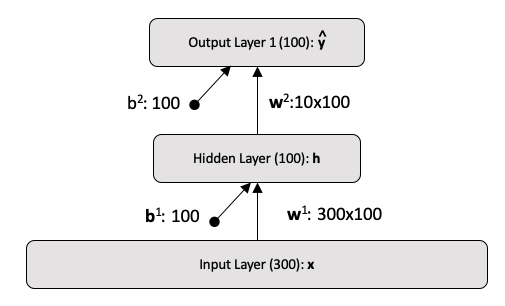
\includegraphics[width=3in]{figure1.png}
\end{center}

The data set we are using for this problem consists of one-lead echocardiogram (ECG) traces\footnote{See \url{https://en.wikipedia.org/wiki/Electrocardiography}}. These data have significant structure, but will be very challenging to predict accurately. This problem has not been investigated on this data set previously, so optimal architectures are not known, nor is the floor for achievable loss values. \\

\newpart{10}~~Starting from the provided template (\verb|nn.py|), implement a Scikit-Learn compatible class for the model shown above. You will develop your implementation using NumPy and PyTorch. You are strongly encouraged to use automatic differentiation methods to develop your implementation. In the implementation of \verb|fit| for this question, use the RMSprop optimizer included with PyTorch. Use a learning rate of $1e-3$ and the RMSprop optimizer's built-in weight decay set to $1e-4$ and momentum set to $0.9$. You should learn the model using a batch size equal to the full training set size.\\

\newpart{5} ~Using the provided training data set, learn the model for 400 epochs (in this case epochs and iterations are the same as we are learning the model on full batches). Report the loss on both the training and validation sets.\\

\newpart{5} ~Provide line plots of the first five validation set outputs and their corresponding predictions. There should be one plot per validation case showing the true and predicted time series values. Be sure to provide a legend and axis labels.\\

\end{problem}


\begin{problem}{60} \textbf{More Neural Networks:} 
In this problem, your task is to attempt to improve on the performance of the model and learning approach presented in Question 2. You can make any modifications that you like to the model or the learning algorithm, but the best model you select is limited to one minute of compute time per epoch as measured in the Gradescope autograding environment.  \\

\newpart{20}~~Begin by exploring different models and/or algorithms for this problem. You must try at least one CNN and one RNN architecture. Describe at a high level the different architectures and/or algorithm choices that you tried. Summarize your results using tables or figures. Upload the code for one of your RNN and one of your CNN architectures in \verb|rnn.py| and \verb|cnn.py|. 
 \\

\newpart{10}~~Next, you will need to select a single best model/algorithm combination among the choices you explored in part (a). As your answer to this question, describe what experimental procedures you used to select the single best model. Also describe why you selected this approach. \\

\newpart{5} For the single best model that you selected, provide an architecture diagram (similar to the one shown above) or specify your architecture in detail using equations (Note: this question is not asking you to include a listing of the PyTorch code defining your model in your report). Upload code for your best model in \verb|best_nn.py|.\\

\newpart{10}~~Describe all details of the learning algorithm used for your best model. How did you select final values for any hyperparameters?\\  

\newpart{5} ~Provide line plots of the first five validation test cases and their predictions using your best model. There should be one plot per validation case showing the true and predicted time series values. Be sure to provide a legend and axis labels.\\

\newpart{10} Using the provided test data, compute predictions for all test data cases. Save a Numpy array of predictions to your  code folder using \verb|np.save("predictions.npy", ...)|. Upload the prediction file to Gradescope for scoring.  (Note: point allocations for this question will be based on the performance of your best model relative to an improved baseline model developed by the course staff, as well as to the best solutions found by other students in the class). 

\end{problem}

\showpoints
\end{document}
